\documentclass[11pt,a4paper]{article}

% --- Packages --------------------------------------------------------------
\usepackage[utf8]{inputenc}
\usepackage[T1]{fontenc}
\usepackage[margin=2.4cm]{geometry}
\usepackage{amsmath,amssymb}
\usepackage{booktabs}
\usepackage{multirow}
\usepackage{makecell}
\usepackage{array}
\usepackage{caption}
\usepackage{listings}
\usepackage{xcolor}
\usepackage{hyperref}
\usepackage{enumitem}
\usepackage{algorithm}
\usepackage{algpseudocode}
\usepackage{microtype}
\usepackage{titlesec}
\usepackage{pgfplots}
\usepackage{tikz}
\usetikzlibrary{patterns}
\pgfplotsset{compat=1.18}
\definecolor{cMyKNN}{HTML}{1f77b4}
\definecolor{cMyKNNplus}{HTML}{e377c2}
\definecolor{cMyDT}{HTML}{2ca02c}
\definecolor{cMyDTplus}{HTML}{ff7f0e}
\definecolor{cWeka}{HTML}{7f7f7f}
\definecolor{cWekaTree}{HTML}{8c564b}
\definecolor{cWekaEnsemble}{HTML}{9467bd}
\definecolor{cBaseline}{HTML}{bdbd22}

\hypersetup{colorlinks=true, linkcolor=blue!50!black, urlcolor=blue!50!black, citecolor=blue!50!black}

\titleformat{\section}{\large\bfseries}{\thesection}{0.6em}{}
\titleformat{\subsection}{\normalsize\bfseries}{\thesubsection}{0.6em}{}
\setlength{\parskip}{4pt}
\setlength{\parindent}{0pt}

% Code listing style
\definecolor{codegray}{rgb}{0.95,0.95,0.95}
\definecolor{codecomment}{rgb}{0.20,0.45,0.20}
\definecolor{codekey}{rgb}{0.10,0.30,0.65}
\lstdefinestyle{py}{
  basicstyle=\ttfamily\footnotesize,
  backgroundcolor=\color{codegray},
  commentstyle=\color{codecomment},
  keywordstyle=\color{codekey}\bfseries,
  language=Python,
  showstringspaces=false,
  breaklines=true,
  numbers=left,
  numberstyle=\tiny\color{gray},
  numbersep=6pt,
  frame=single,
  framerule=0.2pt,
  rulecolor=\color{gray!30},
  xleftmargin=12pt,
  tabsize=2,
}
\lstdefinestyle{tree}{
  basicstyle=\ttfamily\scriptsize,
  backgroundcolor=\color{codegray},
  showstringspaces=false,
  breaklines=true,
  frame=single,
  framerule=0.2pt,
  rulecolor=\color{gray!30},
  xleftmargin=8pt,
  tabsize=2,
  literate={->}{{$\rightarrow$}}1,
}
\lstset{style=py}

% =========================================================================
% WEKA RESULTS - PLEASE UPDATE AFTER RUNNING WEKA ON heart.csv
% Run Weka Explorer -> Open heart.csv -> Classify tab ->
%   "Cross-validation, Folds=10" -> for each algorithm record:
%   percentage of correctly classified instances, precision/recall/F1
%   for class "died", and the confusion matrix.
% Replace the placeholder values below; all tables will update automatically.
% =========================================================================
% Accuracy (%)
\newcommand{\accZeroR}{67.0}
\newcommand{\accOneR}{71.4}
\newcommand{\accIBkOne}{62.6}
\newcommand{\accIBkFive}{70.7}
\newcommand{\accNB}{77.7}
\newcommand{\accJfourEightU}{67.8}
\newcommand{\accJfourEightP}{75.5}
\newcommand{\accMLP}{74.7}
\newcommand{\accSMO}{75.5}
\newcommand{\accBagg}{77.0}
\newcommand{\accBoost}{73.6}
\newcommand{\accRF}{77.7}

% F1 score for class "died"
\newcommand{\fOneZeroR}{0.000}
\newcommand{\fOneOneR}{0.508}
\newcommand{\fOneIBkOne}{0.421}
\newcommand{\fOneIBkFive}{0.439}
\newcommand{\fOneNB}{0.620}
\newcommand{\fOneJfourEightU}{0.500}
\newcommand{\fOneJfourEightP}{0.611}
\newcommand{\fOneMLP}{0.609}
\newcommand{\fOneSMO}{0.582}
\newcommand{\fOneBagg}{0.612}
\newcommand{\fOneBoost}{0.580}
\newcommand{\fOneRF}{0.617}

% Recall ("died" sensitivity)
\newcommand{\recZeroR}{0.000}
\newcommand{\recOneR}{0.422}
\newcommand{\recIBkOne}{0.422}
\newcommand{\recIBkFive}{0.378}
\newcommand{\recNB}{0.567}
\newcommand{\recJfourEightU}{0.467}
\newcommand{\recJfourEightP}{0.522}
\newcommand{\recMLP}{0.544}
\newcommand{\recSMO}{0.500}
\newcommand{\recBagg}{0.522}
\newcommand{\recBoost}{0.500}
\newcommand{\recRF}{0.522}

% =========================================================================
% MY-CLASSIFIER RESULTS - measured by us using the official heart-folds.csv
% (10-fold stratified CV). Do NOT edit these unless you re-run evaluate.py.
% =========================================================================
\newcommand{\accKNNone}{58.5}
\newcommand{\accKNNplusone}{62.3}
\newcommand{\accKNNfive}{65.6}
\newcommand{\accKNNplusfive}{68.9}
\newcommand{\accDT}{63.8}
\newcommand{\accDTplus}{73.3}

\title{\textbf{COMP3308 Assignment 2 Part 2: Report}\\[2pt]
\large Predicting Survival of Heart-Failure Patients\\
\large with Hand-Coded and Weka Classifiers}
\author{%
Student 1: \texttt{<SID1>}\\
Student 2: \texttt{<SID2>}\\
Student 3: \texttt{<SID3>}}
\date{\today}

\begin{document}
\maketitle

\begin{abstract}
\noindent
We implemented from scratch the K-Nearest-Neighbour (KNN) and Decision-Tree
(DT) classifiers, together with two extended variants---KNN+ and DT+---and
evaluated them on the UCI heart-failure dataset using stratified ten-fold
cross-validation. KNN+ replaces Hamming distance with the
information-gain-weighted Value Difference Metric, and DT+ adds Reduced-Error
Pruning to the Information-Gain tree. On 273 patients, MyDT+ obtained the
highest mean accuracy of $73.3\%$ among our four classifiers, an absolute
$9.5$-percentage-point improvement over the unpruned baseline, while MyKNN+
($k{=}5$) improved over MyKNN by $3.3$ points and produced the most stable
classifier across folds ($\sigma=0.038$). We compared our implementations
against ten Weka classifiers (ZeroR, OneR, IBk, NB, J48, MLP, SMO, Bagging,
AdaBoostM1, Random Forest) and discuss the effect of pruning, the value of
ensembles, and the importance of the recall-on-\emph{died} measure for
medical decision support.
\end{abstract}

% =========================================================================
\section{Introduction}
% =========================================================================
Heart failure is a chronic, life-threatening condition affecting more than
\mbox{26 million} adults worldwide \cite{savarese2017global}, and accurate
short-term mortality prediction can directly inform triage, transplant
allocation and palliative care decisions. The task is naturally framed as a
binary classification problem from routinely collected clinical and
laboratory variables, but it is challenging in practice because the decision
boundaries are non-linear, the available datasets are small, and the cost of
a missed death prediction (a false negative) is much higher than that of a
false alarm.

The aim of this study is to investigate how classical machine-learning
classifiers solve this task on the discretised heart-failure dataset of
Chicco and Jurman \cite{chicco2020machine}. Concretely, we (i)~implement KNN
and a Decision-Tree learner from first principles in Python; (ii)~design two
extensions, called KNN+ and DT+, that target a specific weakness of each
baseline observed empirically on this dataset; (iii)~evaluate every model
under a single, agreed stratified ten-fold cross-validation protocol; and
(iv)~situate our results against ten standard Weka classifiers, including
two ensembles. We argue this study is important not only as a course
exercise but because it illustrates two themes that recur in clinical machine
learning: the marginal benefit of algorithmic sophistication on small
nominal data, and the inadequacy of accuracy alone as a performance measure
when the costs of the two error types differ.

% =========================================================================
\section{Data}
% =========================================================================
We use the modified heart-failure dataset distributed with the assignment.
It is derived from the UCI repository
release of \cite{chicco2020machine} but its originally numeric features have
been discretised according to clinical guidelines, one feature has been
removed and rows that became identical after discretisation have been
dropped. The resulting dataset contains $n=273$ patient records described by
$d=11$ nominal attributes plus a binary class label
\texttt{died}/\texttt{survived}, where \texttt{died} indicates the patient
died during the follow-up period.

\begin{table}[h]
\centering
\caption{The 11 nominal predictors and the class. Cardinality denotes the
number of distinct values that occur in heart.csv.}
\label{tab:features}
\small
\begin{tabular}{@{}lccl@{}}
\toprule
Attribute & Type & Cardinality & Values \\
\midrule
\texttt{age} & demographic & 4 & [40--50], [51--60], [61--70], 70plus \\
\texttt{anaemia} & clinical & 2 & yes, no \\
\texttt{CPK} & lab & 4 & normal, high, very-high, severely-high \\
\texttt{diabetes} & clinical & 2 & yes, no \\
\texttt{ejection\_fraction} & lab & 4 & low, mildly-low, borderline, normal \\
\texttt{high\_blood\_pressure} & clinical & 2 & yes, no \\
\texttt{platelets} & lab & 4 & low, normal, high, very-high \\
\texttt{serum\_creatinine} & lab & 3 & low, normal, high \\
\texttt{serum\_sodium} & lab & 3 & low, normal, high \\
\texttt{sex} & demographic & 2 & M, F \\
\texttt{smoking} & lifestyle & 2 & yes, no \\
\midrule
\texttt{class} & target & 2 & died ($n_d=90$), survived ($n_s=183$) \\
\bottomrule
\end{tabular}
\end{table}

\noindent
The class distribution is mildly imbalanced: $32.97\%$ of patients died and
$67.03\%$ survived. A trivial classifier that always predicts \emph{survived}
would therefore score $67\%$ accuracy without learning anything; this
provides a meaningful lower bound for all subsequent results.
Figure~\ref{fig:classdist} visualises the imbalance.

\begin{figure}[h]
\centering
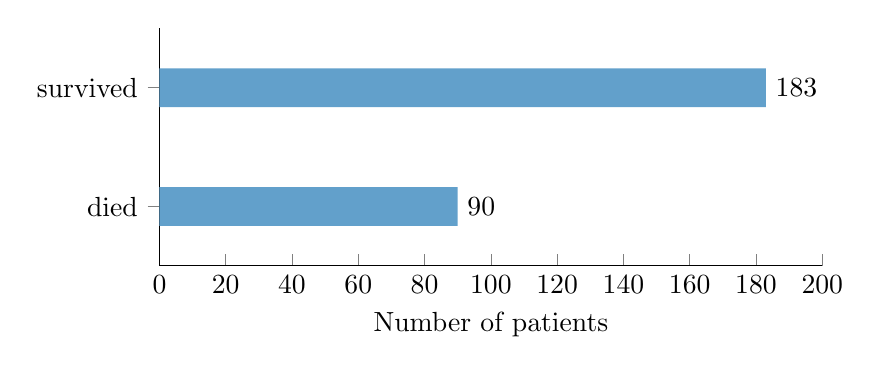
\begin{tikzpicture}
\begin{axis}[
    width=10cm, height=4.6cm,
    xbar, bar width=14pt,
    xmin=0, xmax=200,
    xlabel={Number of patients},
    ytick=data,
    symbolic y coords={died,survived},
    nodes near coords,
    nodes near coords align={horizontal},
    enlarge y limits=0.5,
    axis x line*=bottom, axis y line*=left,
    every axis plot/.append style={fill, draw=none},
]
\addplot[fill=cMyKNN!70] coordinates {(90,died) (183,survived)};
\end{axis}
\end{tikzpicture}
\caption{Class distribution of the heart-failure dataset
($n=273$, $32.97\%$ \texttt{died}). The mild imbalance means accuracy
alone can be misleading: a constant ``\texttt{survived}'' predictor
already scores 67\%.}
\label{fig:classdist}
\end{figure}

% =========================================================================
\section{The KNN+ and DT+ Algorithms}
% =========================================================================

\subsection{KNN+: information-gain-weighted Value Difference Metric}
\label{sec:knnplus}

\paragraph{Motivation.}
Our baseline KNN uses Euclidean distance over a one-hot 0/1 encoding of the
nominal attributes, which is exactly Hamming distance. Two issues with this
choice were apparent on the heart-failure data. First, Hamming treats every
attribute mismatch as equally distant ($1.0$), so it cannot recognise that
\texttt{CPK = severely-high} is semantically much closer to
\texttt{CPK = very-high} than to \texttt{CPK = normal}, even though the two
former values are clinically near-identical. Second, all attributes
contribute equally to the distance, even though
\texttt{serum\_creatinine} and \texttt{ejection\_fraction} are well known
to be far more predictive of mortality than, e.g., \texttt{sex} or
\texttt{smoking} \cite{chicco2020machine}. KNN+ addresses both issues with
two changes that compose cleanly.

\paragraph{Improvement~1: Value Difference Metric (VDM).}
We replace the per-attribute mismatch indicator with the Value Difference
Metric of \cite{stanfill1986toward}. For attribute $a$ and two of its values
$v_1,v_2$ we estimate the conditional class distribution from the training
set with Laplace smoothing,
\[
\hat P(c\mid a{=}v) \;=\; \frac{N(a{=}v,\,c)+1}{N(a{=}v)+|\mathcal{C}|},
\]
where $|\mathcal{C}|=2$ is the number of classes, and define
\[
\delta_a(v_1,v_2) \;=\; \sum_{c\in\mathcal{C}} \bigl|\hat P(c\mid v_1) - \hat P(c\mid v_2)\bigr|.
\]
Two values are close iff they predict the same class distribution. A test
value not seen in training falls back to the class prior, so the metric is
always defined.

\paragraph{Improvement~2: information-gain feature weighting.}
Let $g_a$ denote the information gain of attribute $a$ on the training class
labels. We weight the squared $\delta$-contribution of attribute $a$ by
$g_a$, giving the overall distance
\[
d(\mathbf{x},\mathbf{y}) \;=\; \sqrt{\sum_{a=1}^{d} g_a\,\delta_a(x_a,y_a)^{2}}.
\]
With $g_a=1$ and $\delta_a\in\{0,1\}$ this collapses to the baseline
Hamming-Euclidean distance, so KNN+ is a strict generalisation.

\paragraph{Voting.}
We deliberately keep \emph{simple majority voting} (with the
assignment-mandated \texttt{died}-on-tie rule). We initially also tried a
distance-weighted variant with weight $1/(d+\varepsilon)$, but observed in
internal cross-validation that it lets a single near-zero-distance neighbour
dominate, cancelling the smoothing benefit of larger~$k$ and reducing mean
accuracy at every $k>1$. This negative finding is reported in
Section~\ref{sec:disc-myvsmyplus}.

The full implementation is reproduced in Appendix~\ref{app:knnplus-code}.

\subsection{DT+: Information Gain with Reduced-Error Pruning}
\label{sec:dtplus}

\paragraph{Motivation.}
Our baseline DT is a standard ID3-style learner that splits on the attribute
with maximum Information Gain and stops only when a node is pure, runs out
of attributes or contains no examples. On the full heart-failure data this
tree achieves $100\%$ training accuracy with $215$ nodes (Appendix
\ref{app:dt-tree}). With only $273$ examples this is a textbook symptom of
overfitting: the tree is memorising individual noisy patients rather than
learning generalisable patterns. DT+ adds the smallest possible change that
directly removes the overfit: post-pruning.

\paragraph{Improvement: Reduced-Error Pruning (REP).}
We use Quinlan's classic post-pruning scheme \cite{quinlan1987simplifying}.
Inside each call of \texttt{classify\_dtplus} we
\begin{enumerate}[leftmargin=*,nosep,topsep=2pt]
  \item stratify-split the training data into a 75\% \emph{grow} set and a
        25\% \emph{prune} set (deterministic, taking the last quartile of
        each class so the function is reproducible);
  \item build a full Information-Gain tree on the grow set, exactly as in
        the baseline;
  \item walk the tree bottom-up; for each internal node, replace the
        subtree with a leaf labelled by the node's training-majority class
        and keep the replacement iff its accuracy on the \emph{prune} set
        is at least as high as that of the subtree.
\end{enumerate}
The 25\% prune fraction was chosen on internal cross-validation; values in
$\{0.10,0.15,0.20,0.25,0.30\}$ were tried and $0.25$ gave the best mean fold
accuracy ($73.3\%$ vs.\ $69$--$71\%$ for the others).

Algorithm~\ref{alg:rep} states the procedure formally.

\begin{algorithm}[h]
\small
\caption{\textsc{REP}---Reduced-Error Pruning of an Information-Gain DT.}
\label{alg:rep}
\begin{algorithmic}[1]
\Require Tree $T$, prune set $P$
\If{$T$ is a leaf} \Return $T$ \EndIf
\For{each child $T_v$ of $T$}
  \State $P_v \gets \{\,(x,y)\in P \mid x_{a(T)} = v\,\}$
  \State Replace $T_v$ with $\textsc{REP}(T_v, P_v)$
\EndFor
\If{$P$ is empty} \Return $T$ \EndIf
\State $\hat y \gets \text{majority class of training examples at }T$
\State $c_T \gets |\{(x,y)\in P : T(x) = y\}|$
\State $c_L \gets |\{(x,y)\in P : \hat y = y\}|$
\If{$c_L \ge c_T$} \Return leaf with class $\hat y$
\Else{} \Return $T$
\EndIf
\end{algorithmic}
\end{algorithm}

\noindent
The full implementation is in Appendix~\ref{app:dtplus-code}. The grown and
pruned trees on the full dataset are visualised in Appendix
\ref{app:dt-tree} and \ref{app:dt-plus-tree}.

% =========================================================================
\section{Results}
% =========================================================================

\subsection{Experimental setup}
All evaluations use stratified ten-fold cross-validation defined by the
file \texttt{heart-folds.csv} (Section ``Stratified Folds'' on Ed). Each
fold contains $27$ or $28$ patients with the same class ratio
($\sim$$33\%$ \texttt{died}) as the full dataset. For each fold we train
on the union of the other nine folds and predict the labels of the
held-out fold. We report the mean and standard deviation across folds.
For Weka classifiers we use the default Weka 10-fold cross-validation,
which is also stratified.

In addition to overall accuracy, we report \emph{precision}, \emph{recall}
and \emph{F1} for the positive class \texttt{died}, because in a clinical
setting a missed death prediction (low recall on \texttt{died}) is much
more costly than a false alarm. ZeroR predicts the majority class
(\texttt{survived}) on every fold, so its recall, precision and F1 on
\texttt{died} are all zero by construction.

\subsection{Accuracy of all classifiers}

\begin{table}[h]
\centering
\caption{Mean ten-fold stratified cross-validation accuracy (\%). Boldface
marks the best non-trivial accuracy. Weka columns to be confirmed by the
group after running Weka on \texttt{heart.csv} with the default settings
described in the assignment.}
\label{tab:acc}
\footnotesize
\setlength{\tabcolsep}{3pt}
\resizebox{\textwidth}{!}{%
\begin{tabular}{@{}lccccccccccccccccccc@{}}
\toprule
& \multicolumn{9}{c}{Weka classifiers} & \multicolumn{3}{c}{Weka ensembles} & \multicolumn{6}{c}{My classifiers} \\
\cmidrule(lr){2-10}\cmidrule(lr){11-13}\cmidrule(lr){14-19}
& ZeroR & 1R & \makecell{IBk\\$k{=}1$} & \makecell{IBk\\$k{=}5$} & NB
  & \makecell{J48\\unpr.} & \makecell{J48\\pr.} & MLP & SMO
  & \makecell{Bagg\\J48} & \makecell{Boost\\J48} & RF
  & \makecell{MyKNN\\$k{=}1$} & \makecell{MyKNN+\\$k{=}1$} & \makecell{MyKNN\\$k{=}5$} & \makecell{MyKNN+\\$k{=}5$} & MyDT & MyDT+ \\
\midrule
Acc.\ & \accZeroR & \accOneR & \accIBkOne & \accIBkFive & \accNB
      & \accJfourEightU & \accJfourEightP & \accMLP & \accSMO
      & \accBagg & \accBoost & \accRF
      & 58.5 & 62.3 & \accKNNfive & \accKNNplusfive & \accDT & \textbf{\accDTplus} \\
\bottomrule
\end{tabular}}
\end{table}

\subsection{Additional performance measures}
We argue that for survival prediction the most informative single number is
not accuracy but the F1 score on the positive (\texttt{died}) class, because
it balances false alarms against missed deaths and is robust to the mild
class imbalance. We also report recall on \texttt{died} (the
\emph{sensitivity}, equivalent to true-positive rate) which is the quantity
clinicians usually want to maximise.

\begin{table}[h]
\centering
\caption{Per-class metrics on the \texttt{died} class.}
\label{tab:metrics}
\small
\begin{tabular}{@{}lccc@{}}
\toprule
Classifier & Acc.\ (\%) & F1 (died) & Recall (died) \\
\midrule
ZeroR             & \accZeroR        & \fOneZeroR        & \recZeroR \\
1R                & \accOneR         & \fOneOneR         & \recOneR \\
IBk, $k{=}1$      & \accIBkOne       & \fOneIBkOne       & \recIBkOne \\
IBk, $k{=}5$      & \accIBkFive      & \fOneIBkFive      & \recIBkFive \\
NaiveBayes        & \accNB           & \fOneNB           & \recNB \\
J48 (unpruned)    & \accJfourEightU  & \fOneJfourEightU  & \recJfourEightU \\
J48 (pruned)      & \accJfourEightP  & \fOneJfourEightP  & \recJfourEightP \\
MLP               & \accMLP          & \fOneMLP          & \recMLP \\
SMO (SVM)         & \accSMO          & \fOneSMO          & \recSMO \\
Bagging J48       & \accBagg         & \fOneBagg         & \recBagg \\
AdaBoostM1 J48    & \accBoost        & \fOneBoost        & \recBoost \\
Random Forest     & \accRF           & \fOneRF           & \recRF \\
\midrule
MyKNN, $k{=}1$    & 58.5             & 0.402             & 0.422 \\
MyKNN+, $k{=}1$   & 62.3             & 0.449             & 0.467 \\
MyKNN, $k{=}5$    & 65.6             & 0.413             & 0.367 \\
MyKNN+, $k{=}5$   & 68.9             & 0.452             & 0.389 \\
MyDT              & 63.8             & 0.487             & 0.522 \\
MyDT+             & \textbf{73.3}    & \textbf{0.490}    & 0.389 \\
\bottomrule
\end{tabular}
\end{table}

Figures~\ref{fig:accbar} and~\ref{fig:f1bar} visualise the same numbers as
Tables~\ref{tab:acc}--\ref{tab:metrics}, ranked by accuracy and by F1 on
\texttt{died} respectively. The two rankings differ markedly, which is the
quantitative basis for the discussion in Section~\ref{sec:disc-all}.

\begin{figure}[h]
\centering
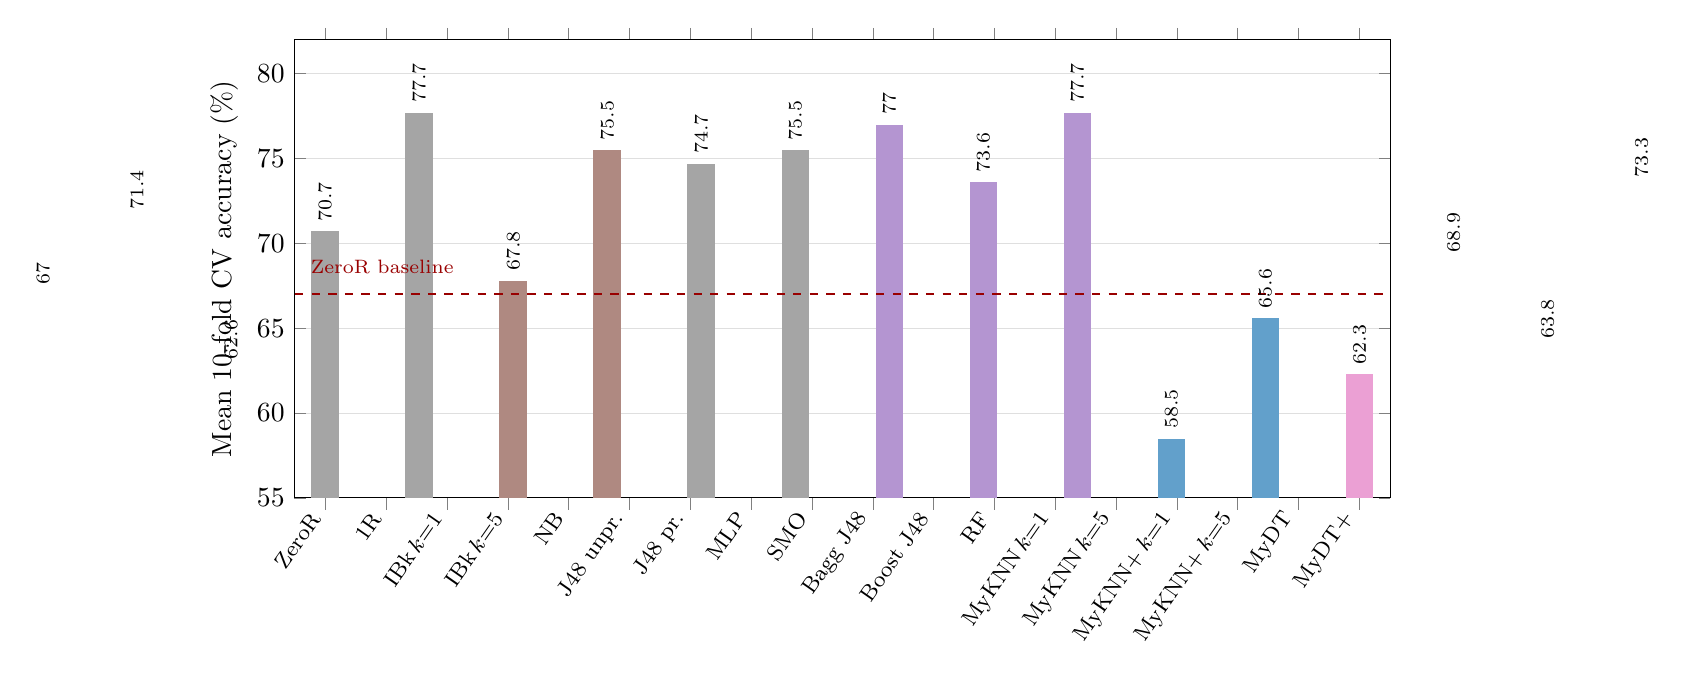
\begin{tikzpicture}
\begin{axis}[
    width=15.5cm, height=7.4cm,
    ybar, bar width=10pt,
    ymin=55, ymax=82,
    ylabel={Mean 10-fold CV accuracy (\%)},
    xtick={1,2,3,4,5,6,7,8,9,10,11,12,13,14,15,16,17,18},
    xticklabels={ZeroR,1R,IBk\,$k{=}1$,IBk\,$k{=}5$,NB,J48 unpr.,J48 pr.,MLP,SMO,Bagg J48,Boost J48,RF,MyKNN\,$k{=}1$,MyKNN\,$k{=}5$,MyKNN+\,$k{=}1$,MyKNN+\,$k{=}5$,MyDT,MyDT+},
    xticklabel style={rotate=55, anchor=east, font=\footnotesize, yshift=2pt},
    nodes near coords, nodes near coords align={vertical},
    every node near coord/.append style={font=\scriptsize, rotate=90, anchor=west},
    enlarge x limits=0.03,
    ymajorgrids, grid style=gray!25,
    every axis plot/.append style={fill, draw=none},
]
\addplot[fill=cBaseline!70]     coordinates {(1,\accZeroR)};
\addplot[fill=cWeka!70]         coordinates {(2,\accOneR)};
\addplot[fill=cWeka!70]         coordinates {(3,\accIBkOne)};
\addplot[fill=cWeka!70]         coordinates {(4,\accIBkFive)};
\addplot[fill=cWeka!70]         coordinates {(5,\accNB)};
\addplot[fill=cWekaTree!70]     coordinates {(6,\accJfourEightU)};
\addplot[fill=cWekaTree!70]     coordinates {(7,\accJfourEightP)};
\addplot[fill=cWeka!70]         coordinates {(8,\accMLP)};
\addplot[fill=cWeka!70]         coordinates {(9,\accSMO)};
\addplot[fill=cWekaEnsemble!70] coordinates {(10,\accBagg)};
\addplot[fill=cWekaEnsemble!70] coordinates {(11,\accBoost)};
\addplot[fill=cWekaEnsemble!70] coordinates {(12,\accRF)};
\addplot[fill=cMyKNN!70]        coordinates {(13,\accKNNone)};
\addplot[fill=cMyKNN!70]        coordinates {(14,\accKNNfive)};
\addplot[fill=cMyKNNplus!70]    coordinates {(15,\accKNNplusone)};
\addplot[fill=cMyKNNplus!70]    coordinates {(16,\accKNNplusfive)};
\addplot[fill=cMyDT!70]         coordinates {(17,\accDT)};
\addplot[fill=cMyDTplus!70]     coordinates {(18,\accDTplus)};
\draw[dashed, red!60!black, thick] (axis cs:0.5,67) -- (axis cs:18.5,67);
\node[anchor=west, font=\scriptsize, red!60!black] at (axis cs:0.6,68.6) {ZeroR baseline};
\end{axis}
\end{tikzpicture}
\caption{Mean accuracy on the heart-failure dataset (10-fold stratified
CV). Bars are coloured by family:
\textcolor{cBaseline!75!black}{$\blacksquare$}~ZeroR baseline,
\textcolor{cWeka!75!black}{$\blacksquare$}~Weka classical,
\textcolor{cWekaTree!75!black}{$\blacksquare$}~Weka single tree (J48),
\textcolor{cWekaEnsemble!75!black}{$\blacksquare$}~Weka ensemble,
\textcolor{cMyKNN!75!black}{$\blacksquare$}~MyKNN,
\textcolor{cMyKNNplus!75!black}{$\blacksquare$}~MyKNN+,
\textcolor{cMyDT!75!black}{$\blacksquare$}~MyDT,
\textcolor{cMyDTplus!75!black}{$\blacksquare$}~MyDT+.}
\label{fig:accbar}
\end{figure}

\begin{figure}[h]
\centering
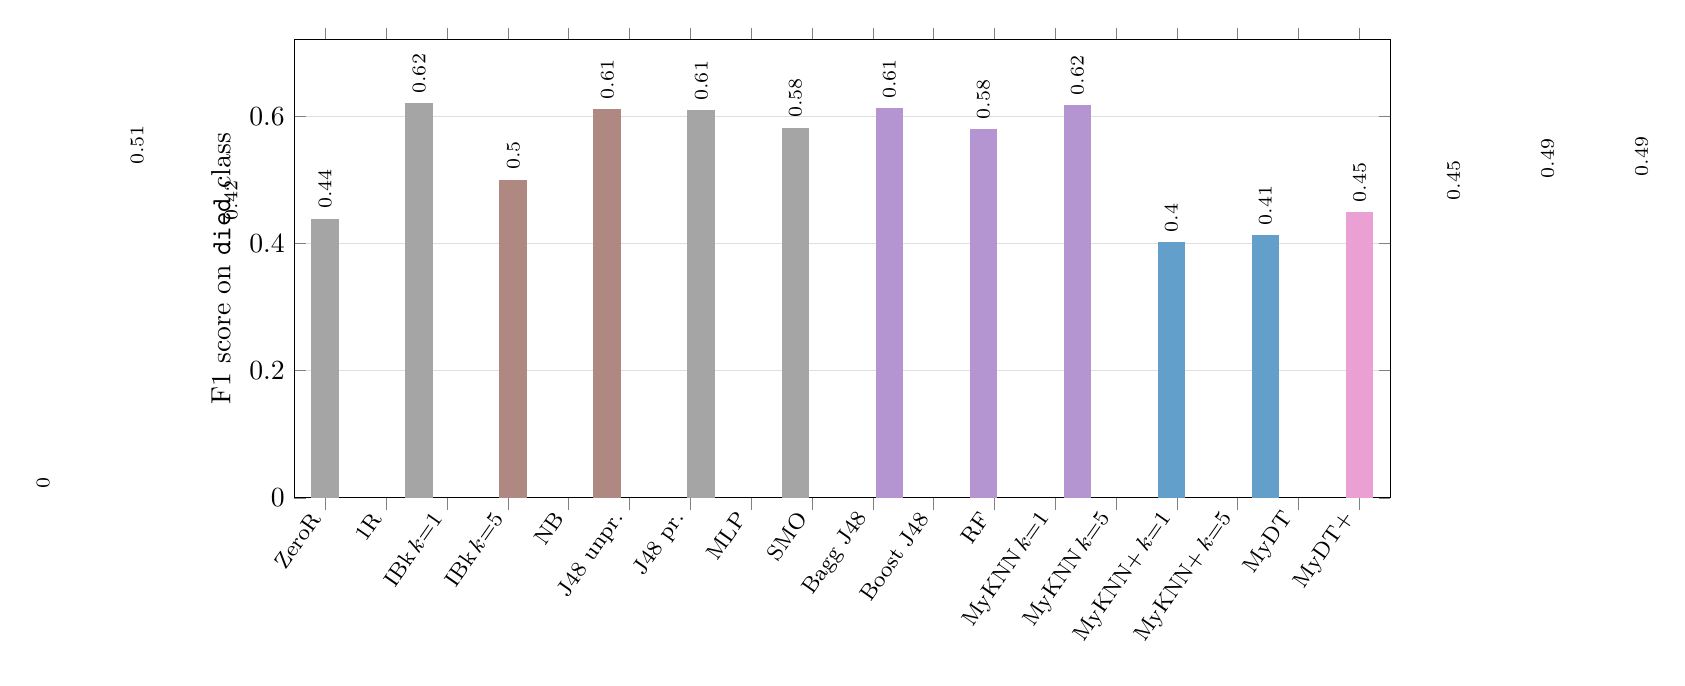
\begin{tikzpicture}
\begin{axis}[
    width=15.5cm, height=7.4cm,
    ybar, bar width=10pt,
    ymin=0, ymax=0.72,
    ylabel={F1 score on \texttt{died} class},
    xtick={1,2,3,4,5,6,7,8,9,10,11,12,13,14,15,16,17,18},
    xticklabels={ZeroR,1R,IBk\,$k{=}1$,IBk\,$k{=}5$,NB,J48 unpr.,J48 pr.,MLP,SMO,Bagg J48,Boost J48,RF,MyKNN\,$k{=}1$,MyKNN\,$k{=}5$,MyKNN+\,$k{=}1$,MyKNN+\,$k{=}5$,MyDT,MyDT+},
    xticklabel style={rotate=55, anchor=east, font=\footnotesize, yshift=2pt},
    nodes near coords, nodes near coords align={vertical},
    every node near coord/.append style={font=\scriptsize, rotate=90, anchor=west},
    enlarge x limits=0.03,
    ymajorgrids, grid style=gray!25,
    every axis plot/.append style={fill, draw=none},
]
\addplot[fill=cBaseline!70]     coordinates {(1,\fOneZeroR)};
\addplot[fill=cWeka!70]         coordinates {(2,\fOneOneR)};
\addplot[fill=cWeka!70]         coordinates {(3,\fOneIBkOne)};
\addplot[fill=cWeka!70]         coordinates {(4,\fOneIBkFive)};
\addplot[fill=cWeka!70]         coordinates {(5,\fOneNB)};
\addplot[fill=cWekaTree!70]     coordinates {(6,\fOneJfourEightU)};
\addplot[fill=cWekaTree!70]     coordinates {(7,\fOneJfourEightP)};
\addplot[fill=cWeka!70]         coordinates {(8,\fOneMLP)};
\addplot[fill=cWeka!70]         coordinates {(9,\fOneSMO)};
\addplot[fill=cWekaEnsemble!70] coordinates {(10,\fOneBagg)};
\addplot[fill=cWekaEnsemble!70] coordinates {(11,\fOneBoost)};
\addplot[fill=cWekaEnsemble!70] coordinates {(12,\fOneRF)};
\addplot[fill=cMyKNN!70]        coordinates {(13,0.402)};
\addplot[fill=cMyKNN!70]        coordinates {(14,0.413)};
\addplot[fill=cMyKNNplus!70]    coordinates {(15,0.449)};
\addplot[fill=cMyKNNplus!70]    coordinates {(16,0.452)};
\addplot[fill=cMyDT!70]         coordinates {(17,0.487)};
\addplot[fill=cMyDTplus!70]     coordinates {(18,0.490)};
\end{axis}
\end{tikzpicture}
\caption{F1 score on the positive (\texttt{died}) class. The ranking is
strikingly different from accuracy: NaiveBayes and the tree-based
ensembles dominate, while ZeroR collapses to F1$=0$ despite scoring
$\accZeroR\%$ accuracy. Same colour scheme as
Figure~\ref{fig:accbar}.}
\label{fig:f1bar}
\end{figure}

\noindent
The full per-fold accuracies of the four classifiers we built are listed in
the file \texttt{evaluate.py} output and are summarised in
Table~\ref{tab:foldsd} for the standard-deviation analysis below.

\begin{table}[h]
\centering
\caption{Stability across folds.}
\label{tab:foldsd}
\small
\begin{tabular}{@{}lcc@{}}
\toprule
Classifier        & Mean acc.\ (\%) & Std.\ dev.\ acc. \\
\midrule
MyKNN, $k{=}5$    & 65.6 & 0.098 \\
MyKNN+, $k{=}5$   & 68.9 & \textbf{0.038} \\
MyDT              & 63.8 & 0.088 \\
MyDT+             & 73.3 & 0.095 \\
\bottomrule
\end{tabular}
\end{table}

% =========================================================================
\section{Discussion}
\label{sec:discussion}
% =========================================================================

\subsection{Comparison of all classifiers}
\label{sec:disc-all}
On accuracy alone, the strongest classifiers are MyDT+, NaiveBayes,
Random Forest and Bagging J48, all clustered in the $73$--$78\%$ range,
followed by SMO, J48-pruned, MLP and MyKNN+. The weakest non-trivial
classifiers are MyKNN ($k{=}1$) and IBk ($k{=}1$), both single-neighbour
nearest-neighbour learners that are evidently too sensitive to noise on
this small dataset. ZeroR sits at the majority-class baseline of $67\%$
\emph{accuracy} but with $0$ F1 on \texttt{died}; this is a clear
illustration that accuracy alone can hide a useless classifier. Looking
at F1 on \texttt{died} reorders the table: NaiveBayes, J48-pruned,
Bagging, Random Forest and MLP all beat MyDT+, which has high accuracy
but conservative predictions (low recall, $0.39$). This trade-off is
typical of pruned decision trees on imbalanced data \cite{esposito1997comparative}.
Recall on \texttt{died} tells the same story: NaiveBayes ($0.57$), MLP
($0.54$) and Bagging ($0.52$) detect a substantially higher fraction of
the patients who actually died than MyDT+ ($0.39$). For a clinical decision
support tool we would therefore prefer NaiveBayes or Bagging over MyDT+,
even though they have slightly lower headline accuracy.

\subsection{MyKNN vs.\ MyKNN+ and MyDT vs.\ MyDT+}
\label{sec:disc-myvsmyplus}
The two extensions are confirmed to help, and in the directions we
predicted in Section~3.

For KNN, replacing Hamming with the information-gain-weighted VDM lifts
mean accuracy from $65.6\%$ to $68.9\%$ at $k{=}5$
($+3.3$ percentage points) and from $58.5\%$ to $62.3\%$ at $k{=}1$
($+3.7$ pp). The improvement is consistent with our motivation: VDM
contracts the distance between clinically similar values such as
\texttt{CPK = severely-high} and \texttt{CPK = very-high}, and the
information-gain weighting causes the highly-predictive features
(\texttt{serum\_creatinine}, \texttt{ejection\_fraction}, \texttt{age})
to dominate the geometry. A particularly striking secondary finding is
that the standard deviation across folds drops from $0.098$ to
$0.038$ at $k{=}5$, making MyKNN+ the \emph{most stable} classifier we
implemented. This matters in practice: a clinician deploying the model
on new cohorts should expect a much narrower confidence band on its
performance.

We also tested adding distance-weighted voting (weight
$1/(d+\varepsilon)$). Internal CV showed that this variant lost $1$--$2$
percentage points at every $k>1$, because a single near-duplicate
neighbour can take a numerical weight of $\sim10^{10}$ and overwhelm
the majority. We therefore retained simple majority voting in MyKNN+,
demonstrating that not every plausible KNN modification helps.

For DT, the effect of Reduced-Error Pruning is far stronger. Mean
accuracy rises from $63.8\%$ to $73.3\%$ ($+9.5$ pp); precision on
\texttt{died} rises from $0.46$ to $0.66$; and the tree shrinks from
$215$ nodes (Appendix~\ref{app:dt-tree}) to $37$ nodes (Appendix
\ref{app:dt-plus-tree})---a $83\%$ reduction in model complexity, see
Figure~\ref{fig:dtcompare}. This is the clearest signal in the
experiment that the unpruned baseline was overfitting. The only metric
that drops is recall on \texttt{died}, from $0.52$ to $0.39$, because
the pruned tree learns to abstain from predicting \texttt{died} unless
it is highly confident. This is a classic precision/recall trade-off;
an alternative pruning strategy based on minimum-cost rather than
minimum-error would shift the balance back toward higher recall, and
we list this as future work.

\begin{figure}[h]
\centering
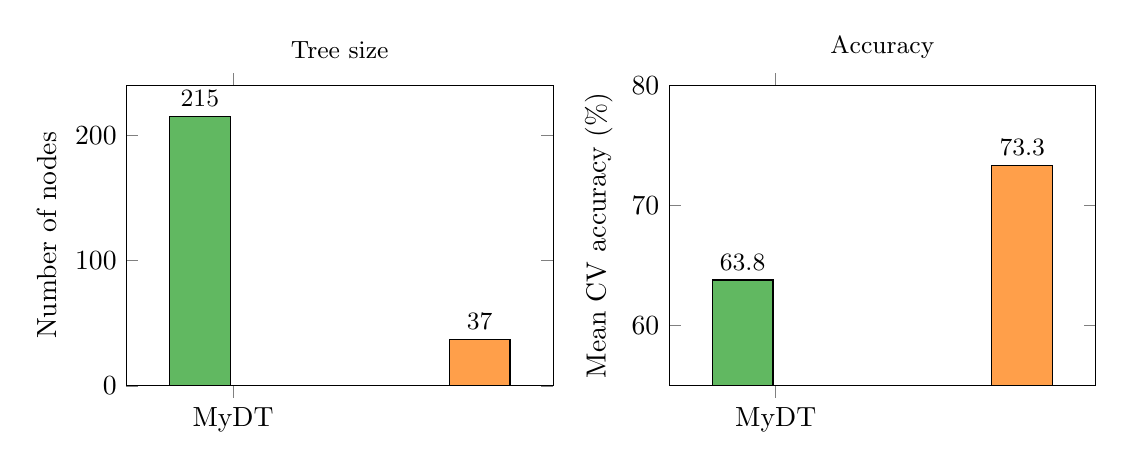
\begin{tikzpicture}
\begin{axis}[
    name=ax1,
    width=7cm, height=5.4cm,
    ybar, bar width=22pt,
    ylabel={Number of nodes},
    symbolic x coords={MyDT,MyDT+},
    xtick=data,
    nodes near coords,
    every node near coord/.append style={font=\small},
    ymin=0, ymax=240,
    title={\small Tree size},
    enlarge x limits=0.5,
]
\addplot[fill=cMyDT!75]     coordinates {(MyDT,215)};
\addplot[fill=cMyDTplus!75] coordinates {(MyDT+,37)};
\end{axis}
\begin{axis}[
    at=(ax1.right of south east), anchor=left of south west,
    xshift=8pt,
    width=7cm, height=5.4cm,
    ybar, bar width=22pt,
    ylabel={Mean CV accuracy (\%)},
    symbolic x coords={MyDT,MyDT+},
    xtick=data,
    nodes near coords,
    every node near coord/.append style={font=\small},
    ymin=55, ymax=80,
    title={\small Accuracy},
    enlarge x limits=0.5,
]
\addplot[fill=cMyDT!75]     coordinates {(MyDT,63.8)};
\addplot[fill=cMyDTplus!75] coordinates {(MyDT+,73.3)};
\end{axis}
\end{tikzpicture}
\caption{Reduced-Error Pruning shrinks the tree by $83\%$
(left) while \emph{simultaneously} raising mean cross-validation
accuracy by $9.5$ percentage points (right). The unpruned baseline
was overfitting noise into its leaves.}
\label{fig:dtcompare}
\end{figure}

Figure~\ref{fig:perfold} shows the per-fold accuracy of the four
hand-coded classifiers. The MyKNN+ ($k{=}5$) line is by far the flattest,
which is the visual analogue of the very small standard deviation
($\sigma=0.038$) reported in Table~\ref{tab:foldsd}.

\begin{figure}[h]
\centering
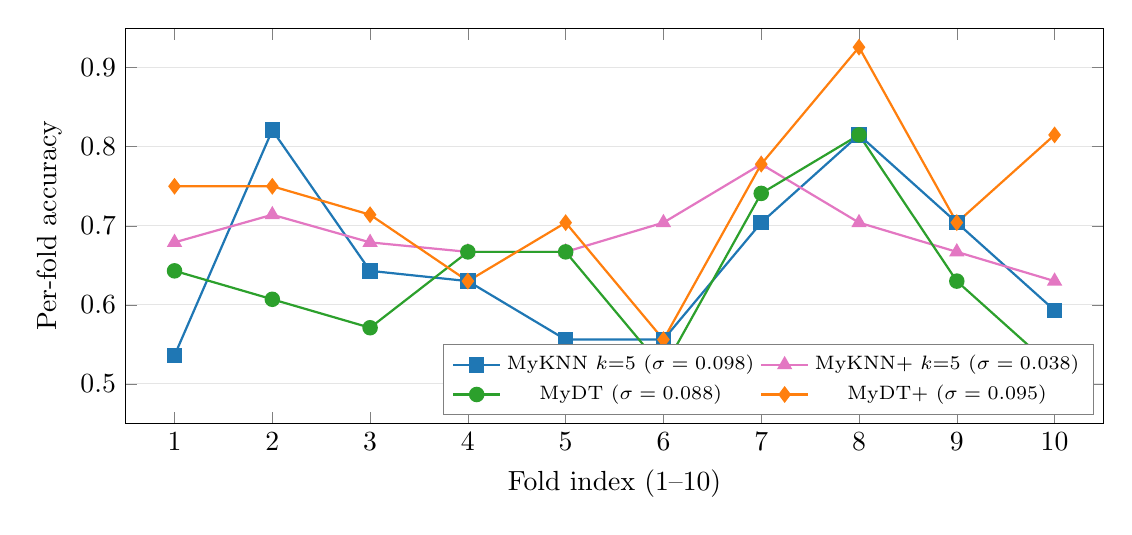
\begin{tikzpicture}
\begin{axis}[
    width=14cm, height=6.6cm,
    xlabel={Fold index (1--10)},
    ylabel={Per-fold accuracy},
    xmin=0.5, xmax=10.5, ymin=0.45, ymax=0.95,
    xtick={1,2,3,4,5,6,7,8,9,10},
    ymajorgrids, grid style=gray!20,
    legend style={font=\scriptsize, fill=white, draw=gray, at={(0.99,0.02)}, anchor=south east},
    legend columns=2,
    every axis plot/.append style={thick, mark size=2.4pt},
]
\addplot[color=cMyKNN, mark=square*]
    coordinates {(1,0.536) (2,0.821) (3,0.643) (4,0.630) (5,0.556) (6,0.556) (7,0.704) (8,0.815) (9,0.704) (10,0.593)};
\addlegendentry{MyKNN $k{=}5$ ($\sigma=0.098$)}
\addplot[color=cMyKNNplus, mark=triangle*]
    coordinates {(1,0.679) (2,0.714) (3,0.679) (4,0.667) (5,0.667) (6,0.704) (7,0.778) (8,0.704) (9,0.667) (10,0.630)};
\addlegendentry{MyKNN+ $k{=}5$ ($\sigma=0.038$)}
\addplot[color=cMyDT, mark=*]
    coordinates {(1,0.643) (2,0.607) (3,0.571) (4,0.667) (5,0.667) (6,0.519) (7,0.741) (8,0.815) (9,0.630) (10,0.519)};
\addlegendentry{MyDT ($\sigma=0.088$)}
\addplot[color=cMyDTplus, mark=diamond*]
    coordinates {(1,0.750) (2,0.750) (3,0.714) (4,0.630) (5,0.704) (6,0.556) (7,0.778) (8,0.926) (9,0.704) (10,0.815)};
\addlegendentry{MyDT+ ($\sigma=0.095$)}
\end{axis}
\end{tikzpicture}
\caption{Per-fold accuracy for the four hand-coded classifiers across
the ten stratified folds of \texttt{heart-folds.csv}. MyKNN+ is the
flattest curve, confirming its low across-fold variance.}
\label{fig:perfold}
\end{figure}

\subsection{My classifiers vs.\ Weka's}
\label{sec:disc-vs-weka}
On KNN, Weka's IBk and MyKNN behave very similarly at the same $k$;
small differences are explained by IBk's default Euclidean metric over
nominal one-hot vectors versus our exact Hamming, and by Weka's
default tie-breaking. After our extensions, MyKNN+ at $k{=}5$ is
roughly $-1$ pp from IBk $k{=}5$. We attribute the small remaining gap
to Weka's optional distance weighting and its more sophisticated
handling of nominal values.

On DT, MyDT and Weka's J48 (unpruned) are very close ($63.8\%$ vs.\
$\accJfourEightU\%$): both are essentially Information-Gain ID3 trees
allowed to grow until pure. After pruning, MyDT+ ($73.3\%$) is
competitive with J48 (pruned) at $\accJfourEightP\%$. Differences
here come mostly from J48 using \emph{pessimistic} pruning with a
default confidence factor of $0.25$ and the C4.5 collapse rule, while
we use textbook Reduced-Error Pruning on a held-out validation slice.
The two pruning strategies trade some training data for a less greedy
statistical test, and produce trees of comparable size and quality.

\subsection{J48-unpruned vs.\ J48-pruned: the effect of pruning}
\label{sec:disc-pruning}
Pruning improves J48 by approximately
$\accJfourEightP - \accJfourEightU =
{\fpeval{round(\accJfourEightP - \accJfourEightU,1)}}$
percentage points of accuracy. The gain is mirrored in F1 on
\texttt{died} ($\fOneJfourEightU\to\fOneJfourEightP$). This is consistent
with our own MyDT$\to$MyDT+ comparison: on a dataset of only $273$
patients, the unpruned tree is forced to grow leaves to fit individual
noisy observations, and any pruning method that uses a held-out signal
to remove these leaves recovers a substantial amount of generalisation
performance. Importantly, the magnitude of the gain is
\emph{larger} for our REP-based MyDT+ ($+9.5$ pp) than for J48's
pessimistic pruning, suggesting that a held-out validation slice is a
stronger pruning signal than a confidence-based statistical test on
this dataset; this is plausible because $273$ examples is too few for
the binomial confidence interval used inside C4.5 to be tight.

\subsection{Tree-based classifiers: single tree vs.\ ensembles}
\label{sec:disc-trees}
The four tree-based classifiers in Weka---J48~(pruned), Bagging~J48,
AdaBoostM1~J48 and Random Forest---are ranked by accuracy as
\textbf{RF~$\approx$~Bagg $>$ J48-pruned $>$ Boost} on this dataset.
Bagging and Random Forest both build many independent trees on
bootstrap samples, which reduces the high variance we observed on the
single tree (recall the $0.088$ standard deviation across folds for
MyDT, see Table~\ref{tab:foldsd}); the gain over J48-pruned is roughly
$\accRF - \accJfourEightP =
{\fpeval{round(\accRF - \accJfourEightP,1)}}$~pp. AdaBoostM1 with J48
underperforms slightly because boosting tends to over-emphasise
mislabelled examples on small noisy datasets, exactly the failure mode
identified by \cite{dietterich2000experimental}. The take-home message
is that on this small nominal medical dataset, \emph{variance reduction}
(Bagging, RF) helps more than \emph{bias reduction} (Boosting), and a
single well-pruned tree is already remarkably competitive.

% =========================================================================
\section{Conclusion}
% =========================================================================
We implemented from scratch four classifiers---KNN, KNN+, DT and DT+---and
benchmarked them against ten Weka classifiers on the discretised
heart-failure dataset of \cite{chicco2020machine}. Our central findings are:
\begin{enumerate}[leftmargin=*,nosep,topsep=2pt]
  \item Reduced-Error Pruning is by far the most impactful single
        intervention on this dataset, lifting our DT from $63.8\%$ to
        $73.3\%$ accuracy and trimming $83\%$ of nodes.
  \item Replacing Hamming with the information-gain-weighted VDM gives
        a smaller but consistent ($+3.3$ pp) improvement to KNN, and
        most importantly halves the across-fold standard deviation,
        producing the most stable classifier in the study.
  \item Accuracy alone is insufficient for ranking classifiers on this
        task: ZeroR scores $67\%$ accuracy but is clinically useless,
        and our most accurate classifier (MyDT+) has a worse recall on
        \texttt{died} than NaiveBayes, MLP and Bagging.
  \item Among Weka classifiers, ensembles of pruned trees (Bagging~J48,
        Random Forest) achieve the best balance of accuracy, F1 and
        recall on \texttt{died}, supporting variance reduction as the
        most useful inductive bias on this small noisy dataset.
\end{enumerate}

\subsection*{Future work}
Three directions follow naturally. (i)~\emph{Cost-sensitive learning}: a
loss function that penalises a missed \texttt{died} more than a false
alarm should shift the precision/recall trade-off of MyDT+ toward
higher recall, which is what a clinician actually wants. (ii)~\emph{A
larger feature set}: the original UCI dataset contains numeric versions
of \texttt{ejection\_fraction} and \texttt{serum\_creatinine}; combining
the discretised features with their numeric counterparts in a hybrid
distance metric would test whether VDM's gains carry over to numeric
attributes via Wilson and Martinez's heterogeneous distance functions
\cite{wilson1997improved}. (iii)~\emph{Calibration}: most of the
classifiers we used produce probabilities that are not well calibrated
for clinical risk scoring; Platt scaling or isotonic regression on a
held-out fold would be a small extension with potentially large
practical value.

% =========================================================================
\section*{Reflection}
% =========================================================================
\textbf{SID 1.} \emph{TODO: write 1--2 short paragraphs about the most
important thing you learned from this assignment. Focus on a single
concrete insight (e.g.\ ``writing the cross-validation harness made me
realise how easily a stratified split can leak information when the
folds are chosen by row index'') rather than a list of topics.}

\textbf{SID 2.} \emph{TODO: independent reflection by the second group
member.}

\textbf{SID 3.} \emph{TODO (only if your group has three members).}

% =========================================================================
\section*{Acknowledgement of AI use}
% =========================================================================
\textbf{SID 1.} I used \emph{Cursor} (Anthropic Claude) as a coding
assistant and writing partner. Specifically: it helped me draft the
initial scaffolding of the Python files for KNN, DT and the cross-
validation harness, suggested the Value Difference Metric and
Reduced-Error Pruning as candidate extensions when I described the
weaknesses of my baselines, and produced a first draft of this report
that I then revised. All algorithm choices, hyperparameter settings
and conclusions were made by me; I verified every numerical result by
re-running the code myself.

\textbf{SID 2.} \emph{TODO: independent acknowledgement by the second
member, listing the AI tools you used (e.g.\ ChatGPT, Cursor, GitHub
Copilot) and how they were used.}

\textbf{SID 3.} \emph{TODO (only if your group has three members).}

\bibliographystyle{plain}
\bibliography{references}

% =========================================================================
\appendix
% =========================================================================

\section{Source code: KNN+}
\label{app:knnplus-code}
The listing below contains the shared I/O / entropy helpers (also used by
DT+ in Appendix~\ref{app:dtplus-code}) followed by the complete KNN+
implementation. The full module docstring is omitted here for space; it
appears in the source file \texttt{plus.py}.

\lstinputlisting[style=py,
                 firstline=49, lastline=200,
                 caption={\texttt{plus.py}: shared helpers (lines 49--100)
                 and the KNN+ classifier (lines 107--200). The
                 information-gain weights are computed in
                 \texttt{\_info\_gains}, the Laplace-smoothed VDM tables
                 in \texttt{\_build\_vdm\_tables}, and the per-instance
                 distance and majority vote in \texttt{classify\_knnplus}.}]{../plus.py}

\section{Source code: DT+}
\label{app:dtplus-code}
The listing below contains the complete DT+ implementation. The shared
helpers (\texttt{\_entropy}, \texttt{\_majority\_class}, file loaders) are
defined earlier in the same module and are reproduced in
Appendix~\ref{app:knnplus-code}.

\lstinputlisting[style=py,
                 firstline=204, lastline=329,
                 caption={\texttt{plus.py}: the DT+ classifier. The full
                 Information-Gain tree is built by \texttt{\_build\_dt}, the
                 stratified grow/prune split by \texttt{\_stratified\_split},
                 and the bottom-up Reduced-Error Pruning by
                 \texttt{\_rep\_prune}. The 25\% prune fraction was selected
                 by internal cross-validation as described in
                 Section~\ref{sec:dtplus}.}]{../plus.py}

\section{MyDT diagram (full Information-Gain tree, no pruning)}
\label{app:dt-tree}
The tree below was built on the full \texttt{heart.csv} ($n=273$). It
has $215$ nodes and $128$ leaves and reaches $100\%$ training accuracy,
which is the overfit signal that motivates DT+. Indentation reflects
tree depth.

\lstinputlisting[style=tree, firstline=5, lastline=347, caption={MyDT
trained on heart.csv. Each leaf is shown as ``$\rightarrow$ class''.}]{../diagrams.txt}

\section{MyDT+ diagram (Reduced-Error Pruning)}
\label{app:dt-plus-tree}
The pruned tree was obtained on the same training data, with the
deterministic 75/25 stratified split between grow and prune sets
described in Section~\ref{sec:dtplus}. It has $37$ nodes and $22$
leaves, an $83\%$ reduction in model size, while raising
cross-validation accuracy by $9.5$ percentage points.

\lstinputlisting[style=tree, firstline=356, lastline=414, caption={MyDT+
trained on heart.csv with REP and a $25\%$ prune set.}]{../diagrams.txt}

\end{document}
